\documentclass[12pt,letter]{article}
\usepackage[moduleName={Infinite Stairs}]{KautenjaDSP}
\begin{document}
\titlePage{img/Logo}{img/Module}{img/KautenjaDSP}

% -------------------
% MARK: Overview
% -------------------

\section{Overview}

Blocks is a port of the digital oscillator code from the \href{https://mutable-instruments.net/modules/edges/}{Mutable Instruments Edges Module}. Blocks contains four identical channels, each with a sine, triangle, quantized triangle, sample and hold, short LFSR, and long LFSR oscillator.
\begin{itemize}
\item \textbf{Quad wave generator:} Quad 16-bit wave generators with six different shapes
\item \textbf{Quantized triangle wave generator:} Generate NES style triangle wave with 16 steps of quantization
\item \textbf{Noise generator:} generate pseudo-random numbers using sample and hold and short and long LFSRs
\end{itemize}

% -------------------
% MARK: Panel Layout
% -------------------

\clearpage
\section{Panel Layout}

\begin{figure}[!htp]
\centering
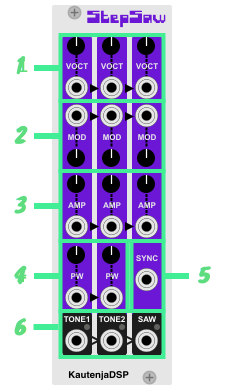
\includegraphics{img/Interface}
\end{figure}

\subsection{Frequency}

The trimpot controls the coarse frequency of the three waveform generators. The ports provide an exponential $V$/Octave input for controlling the pitch of the waveform generators. Inputs are normalled forward from waveform generator one through four.

\subsection{Frequency Modulation}

When nothing is patched to the frequency modulation port, the trimpot can be used to fine tune the frequency of the given waveform generator. When a signal is patched, the input port provides linear frequency modulation to the corresponding waveform generator and the trimpot can be used as an attenuverter to attenuate / polarize the incoming signal. Inputs are normalled forward from waveform generator one through four.

\subsection{Amplifier}

When no input is connected, the trimpot controls the given waveform generator volume level with 8-bit resolution (i.e., $\in [0, 255]$). When an input is patched to the port, the trimpot acts like an attenuator that scales the CV control over the volume level. Because the amplifier has 8-bit control, the envelope of the voice will sound quantized when used with an external envelope generator. Inputs are normalled forward from waveform generator one through four.

\subsection{Shapes}

The \textbf{SHAPE} button cycles between the 6 shapes of the digital oscillator listed by Table~\ref{tab:oscillator-shapes}. The LED provides an indication of the current shape.

\begin{table}[!htp]
\centering
\caption{The shapes of the digital oscillatos.}
\label{tab:oscillator-shapes}
\begin{tabular}{|c|l|}
\hline
 \bfseries Color                                           & \bfseries Shape     \\
\hline\hline
%  \tikz\draw[black,fill=black] (0,0) circle (1ex);          &                     \\
% \hline
 \tikz\draw[black,fill=blue!70!white] (0,0) circle (1ex);  & Sine                \\
\hline
 \tikz\draw[black,fill=green!60!white] (0,0) circle (1ex); & Triangle            \\
\hline
 \tikz\draw[black,fill=blue!20!white] (0,0) circle (1ex);  & Quantized Triangle  \\
\hline
 \tikz\draw[black,fill=red] (0,0) circle (1ex);            & Sample+Hold         \\
\hline
 \tikz\draw[black,fill=pink] (0,0) circle (1ex);           & Long LFSR           \\
\hline
 \tikz\draw[black,fill=yellow] (0,0) circle (1ex);         & Short LFSR          \\
\hline
%  \tikz\draw[black,fill=white] (0,0) circle (1ex);          & Decay-Attack LFO    \\
% \hline
\end{tabular}
\end{table}

\subsection{Outputs}

Each voice produces an output signal of at most $10V_{pp}$ when the amplifier is maxed out. The individual oscillators cannot be overdriven to produce clipping, distortion, or aliasing. However, outputs are normalled forward into a sum mix where hard clipping \textit{can} occur. Excess clipping will introduce an aliasing effect to the mix. Outputs in the mix are clipped \textit{before} being normalled to the next output. VU meter lights measure the output of individual channels going from off ($-\infty dB$ to $-12dB$), to green ($-12dB$ to $0dB$), and lastly to red ($0dB$ to $3dB$) when clipping begins to occur.

% -------------------
% MARK: Data Sheet
% -------------------

\clearpage
\section{Data Sheet}

\begin{table}[!htp]
\begin{tabular}{|l|l|}
\hline
Type             & Oscillator               \\
\hline
Size             & 10 HP Eurorack           \\
\hline
Depth            & NA                       \\
\hline
Power            & NA                       \\ % 2 x 5 Eurorack
\hline
$+12V$ draw (mA) & 0 mA                     \\
\hline
$-12V$ draw (mA) & 0 mA                     \\
\hline
$+5V$ draw (mA)  & 0 mA                     \\
\hline
Sample Rate      & Programmable             \\
\hline
Bit Depth        & 16-bit                   \\
\hline
\end{tabular}
\end{table}

% -------------------
% MARK: References
% -------------------

\clearpage
\renewcommand\refname{References}
\nocite{*}
\bibliographystyle{apalike}
\bibliography{references}

\end{document}
